%% LyX 1.4.3 created this file.  For more info, see http://www.lyx.org/.
%% Do not edit unless you really know what you are doing.
\documentclass[english]{book}
\usepackage[T1]{fontenc}
\usepackage[latin1]{inputenc}
\usepackage{geometry}
\geometry{verbose,letterpaper,tmargin=1in,bmargin=1in,lmargin=1in,rmargin=1in}
\pagestyle{plain}
\setcounter{secnumdepth}{3}
\setcounter{tocdepth}{3}
\usepackage{array}
\usepackage{float}
\usepackage{color}
\usepackage{graphicx}
\IfFileExists{url.sty}{\usepackage{url}}
                      {\newcommand{\url}{\texttt}}

\makeatletter

%%%%%%%%%%%%%%%%%%%%%%%%%%%%%% LyX specific LaTeX commands.
\newcommand{\noun}[1]{\textsc{#1}}
%% Bold symbol macro for standard LaTeX users
\providecommand{\boldsymbol}[1]{\mbox{\boldmath $#1$}}

%% Because html converters don't know tabularnewline
\providecommand{\tabularnewline}{\\}

%%%%%%%%%%%%%%%%%%%%%%%%%%%%%% Textclass specific LaTeX commands.
\newenvironment{lyxcode}
{\begin{list}{}{
\setlength{\rightmargin}{\leftmargin}
\setlength{\listparindent}{0pt}% needed for AMS classes
\raggedright
\setlength{\itemsep}{0pt}
\setlength{\parsep}{0pt}
\normalfont\ttfamily}%
 \item[]}
{\end{list}}

%%%%%%%%%%%%%%%%%%%%%%%%%%%%%% User specified LaTeX commands.
\usepackage{hyperref}

\usepackage{babel}
\makeatother
\begin{document}
%
\begin{figure}[H]
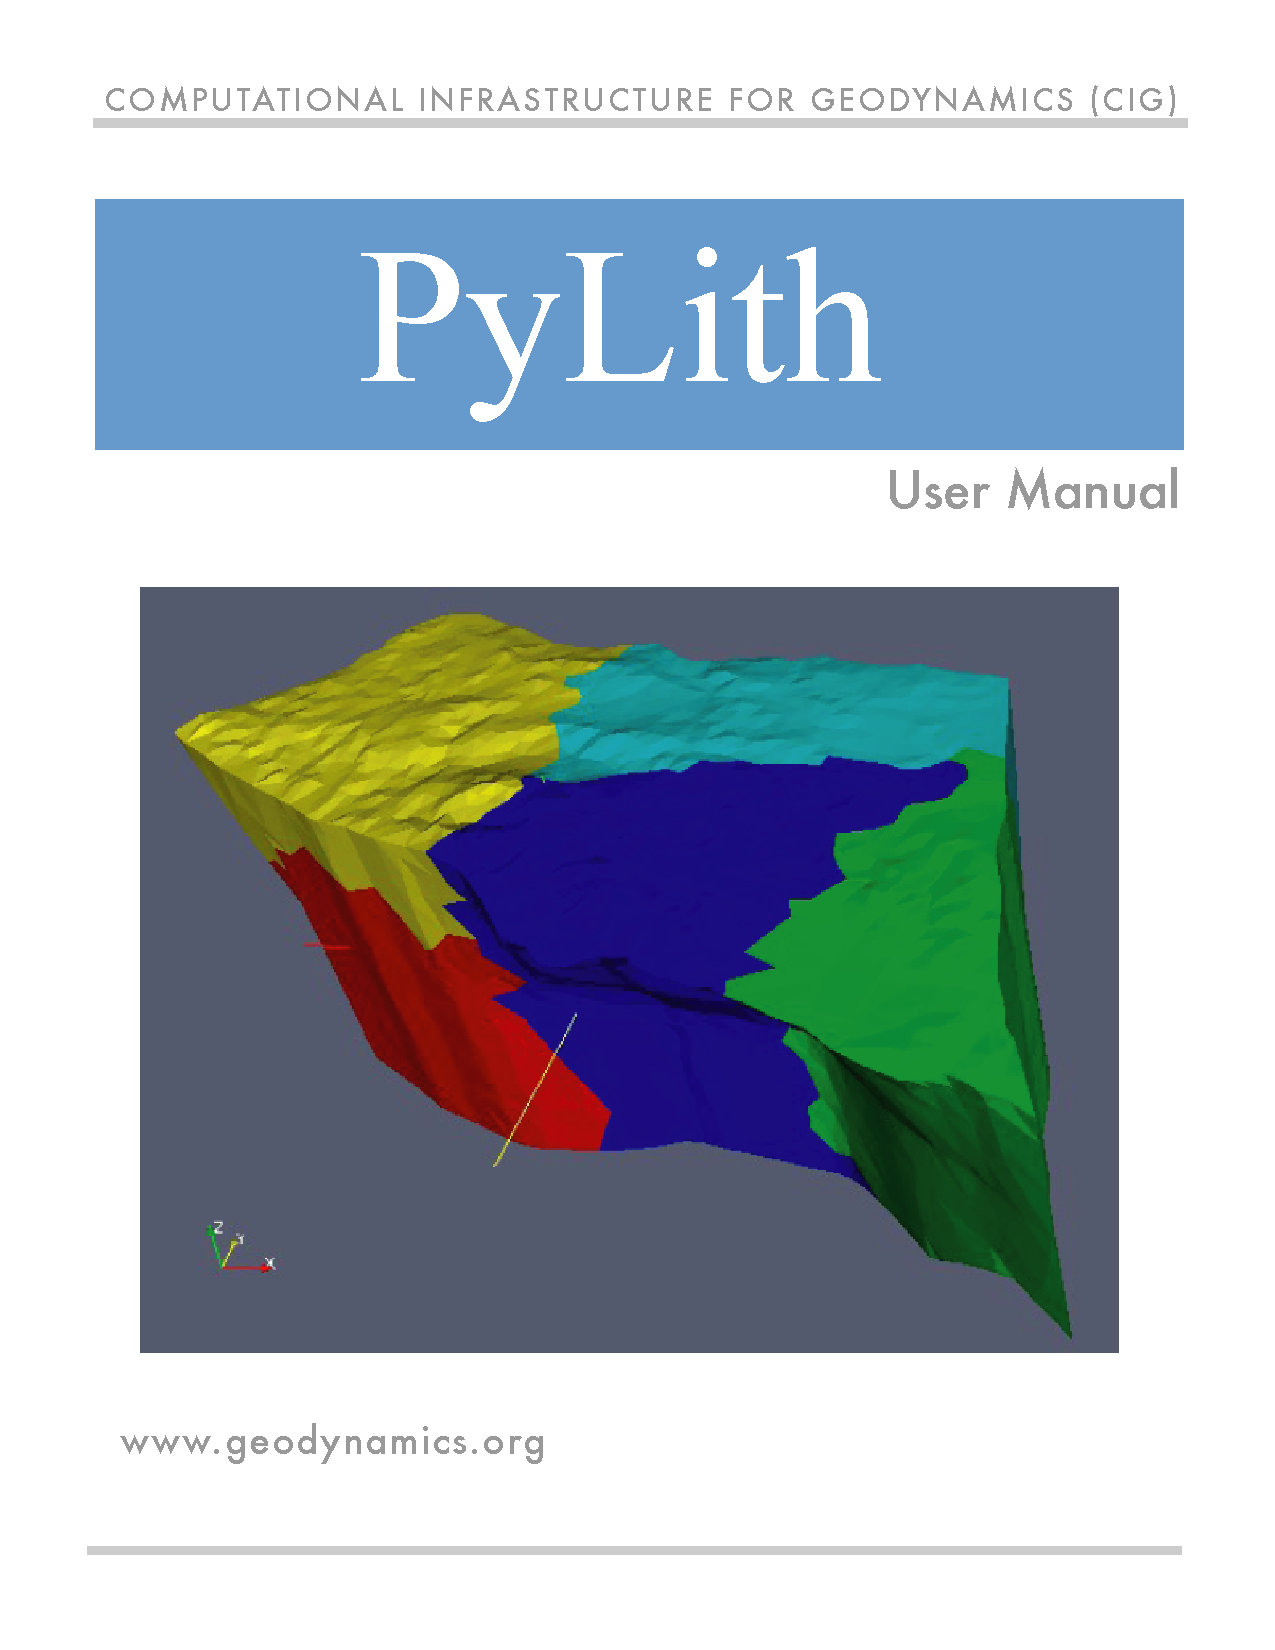
\includegraphics[width=0.75\paperwidth]{pylith_cover}
\end{figure}


\thispagestyle{empty}


\frontmatter

\tableofcontents{}

\listoffigures


\chapter{Preface}

\section{About This Document}

This document is organized into two parts. Part I begins with an
introduction to PyLith and discusses how to run the software. Part II
provides appendices and references.

\section{Who Will Use This Documentation}

This documentation is aimed at scientists who prefer to use
prepackaged and specialized analysis tools. Users are likely to be
experienced computational earth scientists and have familiarity with
basic scripting, software installation, and programming; but are not
likely to be professional programmers. Of those, there are likely to
be two classes of users: those who run models and those who modify the
source code.

\section{Citation}

The Computational Infrastructure for Geodynamics (CIG) is making this
source code available to you at no cost in hopes that the software
will enhance your research in geophysics. A number of individuals have
contributed a significant portion of their careers toward the
development of this software. It is essential that you recognize these
individuals in the normal scientific practice by citing the
appropriate peer reviewed papers and making appropriate
acknowledgements in talks and publications. NEED CITATION INFORMATION

\section{Support}

Current PyLith development is supported by the Southern California
Earthquake Center, the National Science Foundation, the CIG, and
internal U.S. Geological Survey funding. Pyre development is funded by
the \href{http://www.doe.gov/engine/content.do}{Department of
  Energy's} Advanced Simulation and Computing program and the
\href{http://www.nsf.gov}{National Science Foundation's} Information
Technology Research (ITR) program.

\section{Request for Comments}

Your suggestions and corrections can only improve this documentation.
Please report any errors, inaccuracies, or typos to sue (at)
geodynamics.org.


\mainmatter

\chapter{Introduction}

\section{Overview}

PyLith is a multi-scale simulation software package for earthquake
physics. It is portable, scalable software for simulation of crustal
deformation across spatial scales ranging from meters to hundreds of
kilometers and temporal scales ranging from milliseconds to thousands
of years

\section{History}

This first version of PyLith is a direct descendant of Lithomop and
marks the first version that runs in parallel. Lithomop was the
product of major reengineering of Tecton, a finite-element code for
simulating static and quasi-static crustal deformation. The major new
features present in Lithomop included dynamic memory allocation and
the use of the Pyre simulation framework and PETSc solvers. </para>
<para> PyLith is currently being rewritten from scratch to create a
much more modular, powerful simulation package. This new code will
include earthquake dynamics (both rupture propagation and seismic wave
propagation). A beta release is expected in late 2006.

\section{Governing Equations}

Both LithoMop3d and PyLith-0.8 are quasi-static codes, meaning that
time-dependence only enters through the constitutive relationships and
the loading conditions. The description here is for the small-strain
formulation, which is the only formulation available at present. If a
large deformation solution is desired, interested users may contact
Charles Williams (willic3@rpi.edu) about a version of the finite
element code TECTON.

The problem is formulated in terms of the stresses ($\sigma_{ij}$),
displacements ($u_i$), and body forces per unit volume
(figs/g-inlineeq1.eps). We use standard index notation for all
equations here, such that repeated indices imply summation and a comma
denotes differentiation. For a general three-dimensional body, the
problem must satisfy the equilibrium conditions
\begin{equation}
  \text{figs/g-eq1.eps}
\end{equation}
subject to the natural boundary conditions
\begin{equation}
  \text{figs/g-eq2.eps}
\end{equation}
and the essential boundary conditions
\begin{equation}
  \text{figs/g-eq3.eps}
\end{equation}
The surface of the body is $S$, given by
\begin{equation}
  \text{figs/g-eq4.eps}
\end{equation}
The $n_j$ are the components of the unit normal vector to $S$, the
\begin{equation}
  \text{figs/g-inlineeq2.eps}
\end{equation}
are the components of the surface tractions, and the 
\begin{equation}
  \text{figs/g-inlineeq3.eps}
\end{equation}
are the components of the applied displacements. The stresses are
computed from the strains and any existing initial stresses using a
given constitutive relationship. The strains are given by
\begin{equation}
\text{figs/g-eq5.eps}  
\end{equation}
For a linear elastic material, the constitutive relationship between
stress and strain is
\begin{equation}
  \text{figs/g-eq6.eps}
\end{equation}
where
\begin{equation}
  \text{figs/g-inlineeq4.eps}
\end{equation}
are the initial stresses, and $C$
\begin{equation}
  \text{g-inlineeq5.eps}
\end{equation}
is the elastic constitutive relation.

For inelastic behavior (viscous, plastic, etc.), we assume an additive
decomposition of the strain tensor into elastic and inelastic parts,
and use an integrated form of the classical incremental theory of
plasticity. At time $t+\Delta t$, he stresses are therefore computed
from the total elastic strain:
\begin{equation}
  \text{figs/g-eq7.eps}
\end{equation}
where
\begin{equation}
  \text{figs/g-inlineeq6.eps}
\end{equation}
are the total strains and
\begin{equation}
  \text{figs/g-inlineeq7.eps}
\end{equation}
are the inelastic strains, with the difference being the elastic
strains. In our actual computations, we use a formulation that
decomposes the stresses into the deviatoric and volumetric parts,
using ideas based on the "effective stress function"
\cite{Kojic:Bathe:1987}. This allows the time integration of stresses
to be performed in terms of a single parameter related to the second
deviatoric stress invariant.

\section{Software Components}

PyLith is separated into modules to encapsulate behavior and
facilitate use across multiple applications. That way expert users can
replace functionality of a wide variety of components without
recompiling or polluting the main code. External packages reduce
development time and enhance computational efficiency, for example,
PyLith runs 2x faster by using the PETSc linear solver.

PyLith is based on several programming languages. High-level code is
written in Python; this rich, expressive interpreted language with
dynamic typing reduces development time. Low-level code is written in
Fortran 77 for fast execution. Bindings, written in C/C++, are used to
allow the low-level code (Fortran 77) to be called from high-level
code (Python).

PyLith makes extensive use of external software. Pyre is a science
neutral simulation framework being developed at Caltech. PETSc is used
to perform operations on matrices and vectors in parallel.

\subsection{PETSc}

\href{http://www-unix.mcs.anl.gov/petsc/petsc-as/}{PETSc}, the
Portable, Extensible Toolkit for Scientific computation, provides a
suite of routines for parallel, numerical solution of partial
differential equations for linear and nonlinear systems with large,
sparse systems of equations. PETSc includes solvers that implement a
variety of Newton and Krylov subspace methods. It can also interface
with many external packages, including BlockSolve95, ESSL, Matlab,
ParMeTis, PVODE, and SPAI, thereby providing additional solvers and
interaction with other software packages.

PETSc includes interfaces for Fortran, C, and C++ for nearly all of
the routines and PETSc can be installed on most Unix systems. PETSc
can be built with user supplied highly optimized linear algebra
routines (e.g., ATLAS and commercial versions of BLAS/LAPACK), thereby
improving application performance. Users can use PETSc parallel
matrices, vectors, and other data structures for most parallel
operations, eliminating the need for explicit calls to Message Passing
Interface (MPI) routines. Many settings and options can be controlled
with PETSc specific command-line arguments, including selection of
preconditions, solvers, and generation of performance logs.

\subsection{Pyre}

Pyre is an object-oriented environment capable of specifying and
launching numerical simulations on multiple platforms, including
Beowulf class parallel computers and grid computing systems. Pyre
allows the binding of multiple components such as solid and fluid
models used in Earth science simulations, and different meshers. The
Pyre framework enables the elegant setup, modification and launching
of massively parallel three-dimensional solver applications.

Pyre is a framework, a combination of software and design philosophy
that promotes the reuse of code. In their canonical software design
book, {\em Design Patterns}, Erich Gamma {\it et al}.  condense the
concept of a framework concept down to, "When you use a framework, you
reuse the main body and write the code it calls." In the context of
frameworks and object-oriented programming, Pyre can be thought of as
a collection of classes and the way their instances interact.
Programming applications based on Pyre will look similar to those
written in any other object-oriented language. The Pyre framework
contains a subset of parts that make up the overall framework. Each of
those parts is designed to solve a specific problem.

The framework approach to computation offers many advantages. It
permits the exchange of codes and promotes the reuse of standardized
software while preserving efficiency. Frameworks are also an efficient
way to handle changes in computer architecture. They present
programmers and scientists with a unified and well-defined task and
allow for shared costs of the housekeeping aspects of software
development. They provide greater institutional continuity to model
development than piecemeal approaches.


The Pyre framework incorporates features aimed at enabling the
scientific non-expert to perform tasks easily without hindering the
expert. Target features for end users allow complete and intuitive
simulation specification, reasonable defaults, consistency checks of
input, good diagnostics, easy access to remote facilities, and status
monitoring. Target features for developers include easy access to user
input, a shorter development cycle, and good debugging support.

\begin{figure}[htbp]
  \begin{center}
    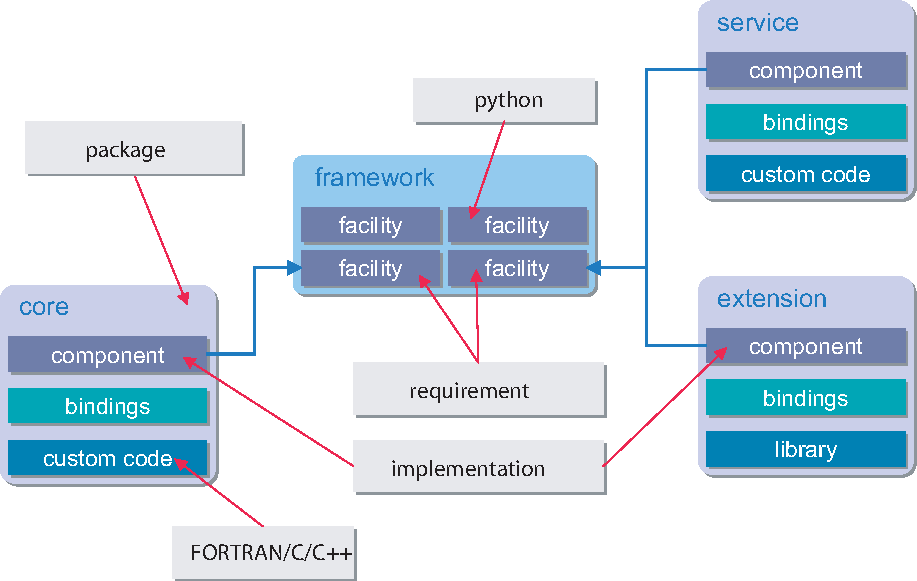
\includegraphics[scale=0.75]{figs/pyre_overview}
    \caption{Pyre Architecture. The integration framework is a set of
      cooperating abstract services.}
  \end{center}
\end{figure}

\section{PyLith Design}

In transforming Lithomop, a serial code, into PyLith, a parallel code,
a principal concern was to preserve the existing structure of the
serial Fortran code. Active development of purely analytic features in
PyLith, such as new material models or discretization schemes, depends
on the familiarity of application scientists with the traditional
Fortran programming paradigm. Global, topological operation should be
strictly segregated from the existing code. In fact, with the
exception of integrating PETSc for serial linear algebra and solver
operations, PyLith can be run purely in serial without activating any
of the parallel capabilities.

In order to accomplish this separation, we use the PETSc
\classname{Sieve} structure to create a model of the serial
PyLith mesh. This model is then partitioned and distributed to a set
of processes. Each process receives a self-consistent mesh, meaning
the pieces are overlapping. Each process then executes a serial PyLith
step on that particular mesh piece. The PETSc linear algebra
operations are overloaded, using the \classname{Sieve}
information, to produce a globally consistent field.

 \chapter{Installation and Getting Help}

\section{Introduction}

Installation of PyLith on a desktop or laptop machine is, in most
cases, very easy. Binary packages have been created for the most
common platforms, including Linux, OSX, and Windows. Installation on
machines that are not compatible with any of these operating systems
requires building the software from the source code, which can be
difficult for inexperienced users.

\section{Getting Help}

Help is available via the CIG Short-Term Crustal Dynamics Mailing List
and CIG's issue tracking system.

\subsection{Requesting help}

The CIG Short-Term Crustal Dynamics Mailing List,
\email{cig-short@geodynamics.org}, is a mailing list dedicated to CIG
issues associated with short-term crustal dynamics, including the use
of PyLith. You can subscribe to the mailing list and view messages at
the \href{http://www.geodynamics.org}{CIG website}.

\subsection{Reporting bugs and errors}

CIG uses the \application{Roundup} for bug tracking. If you find a bug
in PyLith, please submit a bug report to the
\href{http://www.geodynamics.org/roundup}{CIG \application{Roundup}
  system}. Of course, it is helpful to first check to see if someone
else already submitted a report related to the issue; one of the CIG
developers may have already posted a solution to the problem. You can
reply to a current issue by clicking on the issue title. To submit a
new issue, click on \guibutton{Create New} under \guimenu{Issues}.

\section{Installation}

Binary executables are available for three of the most widely used
platforms: 32-bit Linux, Mac OSX, and Windows. If your platform is not
compatible with any of these, you can build the software from the
source code.

\subsection{Linux}

Running the Linux binary version of PyLith requires a 32-bit
compatible machine with GLIBC 2.2 or later.

\begin{enumerate}
\item Download the \href{http://crust.geodynamics.org/~leif/shipping/}{tarball}
\item Unpack the tarball in a suitable location.
  \begin{screen}
    \shellprompt\userinput{tar -zxvf pylith-0.8-linux-x86.tar.gz}
  \end{screen}
\item Add \directory{pylith-0.8-linux-x86/bin} to your \envvar{PATH}.
  You will likely want to add something like
  \begin{screen}
    PATH=\$\{PATH\}:\replaceable{replace\_with\_absolute\_path}/pylith-0.8-linux-x86/bin
  \end{screen}
  to your \filename{.bashrc} file (if you are using bash as your shell)
  or the equivalent to your \filename{.cshrc} file (if you are using
  tcsh as your shell).
\item Add \directory{pylith-0.8-linux-x86/lib}to your
  \envvar{LD\_LIBRARY\_PATH}. You will likely want to add something like
  \begin{screen}
    export LD\_LIBRARY\_PATH=\$\{LD\_LIBRARY\_PATH\}:\replaceable{replace\_with\_}
    \replaceable{absolute\_path}/pylith-0.8-linux-x86/lib
  \end{screen}
  to your \filename{.bashrc} file (if you are using bash as your
  shell) or the equivalent to your \filename{.cshrc} file
  (if you are using tcsh as your shell).
\item To uninstall PyLith, simply remove the \directory{pylith-0.8-linux-x86}
  directory and all of its sub-directories.
\end{enumerate}

\subsection{Mac OSX}

The OSX binary version was built to run on the Macintosh PowerPC
architecture with OSX version 10.2 or later. The binary will run on
the Macintosh Intel architecture, but only in emulation mode (i.e.,
rather slowly).

\begin{enumerate}
\item Download the \href{http://crust.geodynamics.org/~leif/shipping/}{disk image}.
\item Double click on the disk image to mount the disk.
\item Double click on the disk and copy the \directory{PyLith} folder
  to a suiteable location.
\item To run PyLith, double click on the PyLith icon provided in the \directory{PyLith} folder.
\item To uninstall PyLith, simply drag the \directory{PyLith} folder
  to the trash.
\end{enumerate}

\subsection{Windows}

This Windows binary version of PyLith should be compatible with
Windows NT, Windows 2000, and Windows XP.

\begin{enumerate}
\item Download theq
  \href{http://crust.geodynamics.org/~leif/shipping/}{installer}.
\item Double click on the \filename{setup.exe} file you just
  downloaded and follow the instructions for installing.
\item To run PyLith, double click on the PyLith icon on the desktop or
  select
  \guimenu{Start}\guiselect\guimenuitem{All~Programs}\guiselect\guimenuitem{PyLith}\guiselect\guimenuitem{PyLith}.
\item To uninstall PyLith, simply select
  \guimenu{Start}\guiselect\guimenuitem{All
    Programs}\guiselect\guimenuitem{PyLith}\guiselect\guimenuitem{Uninstall~PyLith}.
\end{enumerate}

\section{Building using source tarball}

Building PyLith from the source code is not a trivial task because
PyLith depends on several other packages. In general, each package
must be compiled from source using compilers for each language that
are compatible with one another. The stable version of the PyLith
source code is available from the
\directory{cig/software/Repository/cig/short/3D/PyLith/branches/pylith-0.8}
of the \href{http://www.geodynamics.org:8080/}{Geodynamics subversion
  repository}.

\subsection{System Requirements}

\begin{itemize}
\item Unix flavored operating system.
\item Fortran, C, and C++ compilers.
\item Python (2.3 or later)
\end{itemize}

The software must be built starting from the bottom of the dependency
list and working upwards. The steps below describe the recommended way
to build PyLith and the external packages on which it depends. Some of
the dependencies can be satisfied using precompiled binaries (e.g.,
RedHat and Fink packages). When considering whether to use a
precompiled binary package to satisfy any of the dependencies,
remember that all of the compilers and settings used in building the
code must be compatible.

\begin{enumerate}
\item Build PETSc and MPI.
  \begin{enumerate}
  \item ADD STUFF HERE (LINK TO PETSC SITE? GET MATT'S THOUGHTS ON HOW
    MUCH DETAIL TO PUT HERE)
  \end{enumerate}
\item Build Pythia.
  \begin{enumerate}
  \item ADD STUFF HERE
  \end{enumerate}
\item Build PyLith.
  \begin{enumerate}
  \item ADD STUFF HERE
  \end{enumerate}
\end{enumerate}

\section{Building using source repositories}

\begin{warning}
  Building PyLith using the source repositories is recommended
  only for expert users who are willing to work with a moving
  target and rebuild on a frequent basis. The installation
  instructions cover the basic steps and assume the user has
  experience building and installing software.
\end{warning}

The PyLith-0.8 source code is available from the \href{http://www.geodynamics.org:8080/cig/software/Repository}
\directory{cig/short/3D/PyLith/branches/pylith-0.8}{Geodynamics
  subversion
  repository}.

\subsection{System Requirements}

\begin{itemize}
\item Unix flavored operating system
\item Fortran, C, and C++ compilers
\item Python (2.3 or later)
\item Subversion
\item Mercurial (0.9 or later)
\end{itemize}

\begin{tip}
  Many flavors of Unix have Subversion packages. In most
  cases you do not need anything but the basic subversion
  package. You will likely have to build Mercurial from
  source, but this is a very easy task that takes only a
  couple of minutes.
\end{tip}

\subsection{Building the packages}

The software must be built starting from the bottom of the dependency
list and working upwards. The steps below describe the recommended way
to build PyLith and the external packages on which it depends.

\begin{enumerate}
\item Build
  \href{http://www-unix.mcs.anl.gov/petsc/petsc-as/developers/index.html}{PETSc
    (developers version)} and MPI.
  
  If you have an architecture optimized version of BLAS/LAPACK you
  should use those instead of asking PETSc to download and build one
  for you. In some cases, PETSc will find known optimized
  implementations of BLAS/LAPACK (e.g., vecLib on Mac OSX).
  
  If you have an MPI implementation installed, you can use it or let
  PETSc download and install one for you.

  \begin{tip}
    If you run into problems configuring or building PETSc, send {\em
      both} \filename{configure.log} and
    \filename{make\_\replaceable{PETSC\_ARCH}} to
    \email{petsc-maint@mcs.anl.gov}.
  \end{tip}

  \begin{enumerate}
  \item Pull the source code from ANL and place the source tree in a
    suitable location. The steps below will create a
    \directory{petsc-dev} sub-directory in the current directory.

    \begin{screen}
      \shellprompt\userinput{hg clone http://mercurial.mcs.anl.gov/petsc/petsc-dev}
      \shellprompt\userinput{cd petsc-dev/python}
      \shellprompt\userinput{hg clone http://mercurial.mcs.anl.gov/petsc/BuildSystem BuildSystem}
    \end{screen}
    
  \item Set the \envvar{PETSC\_DIR} and \envvar{PETSC\_ARCH} environment
    variables. \envvar{PETSC\_DIR} corresponds to the top-level
    directory in the PETSc source tree and \envvar{PETSC\_ARCH} is a tag
    for this configuration of PETSc (e.g., linux\_gcc-4.0\_debug,
    darwin\_gcc-3.4\_opt, etc). You will want to set these environment
    variables in your \filename{.bashrc}, \filename{.cshrc}, or
    similar file.

    \begin{screen}
      \shellprompt\userinput{export PETSC\_DIR=\replaceable{replace\_with\_absolute\_path}/petsc-dev}
      \shellprompt\userinput{export PETSC\_ARCH=\replaceable{replace\_with\_PETSc\_arch\_tag}}
    \end{screen}
  \item Configure PETSc.
    
    Run \command{config/configure.py} with the appropriate arguments
    to configure PETSc for your computer. Run
    \command{config/configure.py --help} to see the long list of
    possible options. Building PETSc for use with PyLith requires the
    following arguments:

    \begin{screen}
      \option{--with-clanguage=c++}
      \option{--with-c-support}
      \option{--with-shared=1}
      \option{--with-boost=1}
      \option{--download-boost=1}
      \option{--with-sieve=1}
    \end{screen}
    
    Be sure to include flags indicating where MPI and
    BLAS/LAPACK are if you want to use a preinstalled
    implementation. If not, be sure to tell PETSc to
    download those packages. If you do not want build
    PETSc using the gnu compilers, be sure to let PETSc
    know which compilers you want to use instead.

    After several minutes, the configure script should
    finish and display the PETSc settings. Check to make
    sure these match your expectations before continuing.

  \item Build PETSc.
    \begin{screen}
      \shellprompt\userinput{make}
    \end{screen}
  \item Test PETSc installation.
    
    One of the tests will attempt to display some X windows. If X
    windows is not available from the shell in which you run
    \command{make test}, then that test will fail.

    \begin{screen}
      \shellprompt\userinput{make test}
    \end{screen}
    
  \item In the future, you will likely want to update the PETSc source
    tree to include bug fixes, new features etc.
    
    To update PETSc (use to \command{hg update -v} to see what files
    are being updated):

    \begin{screen}
      \shellprompt\userinput{cd petsc-dev}
      \shellprompt\userinput{hg pull}
      \shellprompt\userinput{hg update}
      \shellprompt\userinput{cd python/BuildSystem}
      \shellprompt\userinput{hg pull}
      \shellprompt\userinput{hg update}
    \end{screen}
  \end{enumerate}

\item Build Pythia.

  \begin{tip}
    If you run into problems configuring or building Pythia, send
    {\em both} the \filename{config.log} and
    \filename{make.log} files to
    \email{cig-short@geodynamics.org}. To create the
    \filename{make.log} file, run make via \command{make $>$ make.log}.
  \end{tip}

  \begin{enumerate}
  \item Pull the source code from CIG and place the source tree in a
    suitable location. The steps below will create a
    \directory{pythia-0.8} sub-directory in the current directory.

    \begin{screen}
      \shellprompt\userinput{svn co svn://geodynamics.org/cig/vendor/pythia [cont.]\\
        /v0.8/pythia-0.8}
    \end{screen}
    
  \item Configure Pythia.
    
    Run \command{configure} with the appropriate arguments.
    Run \command{configure --help} to see a list of possible
    options. You may want to specify compilers and/or an install
    location.

    \begin{screen}
      \shellprompt\userinput{cd pythia-0.8}
      \shellprompt\userinput{autoreconf -i}
      \shellprompt\userinput{./configure}
    \end{screen}

  \item Build Pythia.

    Run \command{make} and \command{make install}.

    \begin{screen}
      \shellprompt\userinput{make}
      \shellprompt\userinput{make install}
    \end{screen}
    
  \end{enumerate}

\item Build PyLith.

  \begin{tip}
    If you run into problems configuring or building PyLith, send
    {\em both} the \filename{config.log} and
    \filename{make.log} files to
    \email{cig-short@geodynamics.org}. To create the
    \filename{make.log} file, run make via \command{make $>$ make.log}.
  \end{tip}

  \begin{enumerate}
  \item Pull the source code from CIG and place the source tree in a
    suitable location. The steps below will create a
    \directory{pylith-0.8} sub-directory in the current directory.

    \begin{screen}
      \shellprompt\userinput{svn co svn://geodynamics.org/cig/short/3D/PyLith [cont.]\\
        /branches/pylith-0.8}
    \end{screen}

  \item Configure PyLith.
    
    Run \command{configure} with the appropriate arguments. Run
    \command{configure --help} to see a list of possible options. You
    may want to specify compilers and/or an install location. If you
    installed pythia-0.8 in a non-system location, you will need to
    set \envvar{CPPFLAGS} and \envvar{LDFLAGS} appropriately.

    \begin{screen}
      \shellprompt\userinput{cd pylith-0.8}
      \shellprompt\userinput{autoreconf -i}
      \shellprompt\userinput{./configure}
    \end{screen}
    
  \item Build PyLith.

    Run \command{make} and \command{make install}.

    \begin{screen}
      \shellprompt\userinput{make}
      \shellprompt\userinput{make install}
    \end{screen}
  \end{enumerate}
\end{enumerate}
 \documentclass[crop,tikz]{standalone}
\usepackage{tikz}
\usetikzlibrary{external}
\tikzexternalize % activate

\begin{document}

\pgfdeclarelayer{background}
\pgfsetlayers{background,main}

\usetikzlibrary{arrows,shapes}
\definecolor{yellow}{rgb}{1.0, 1.0, 0.45} % 255/255/115
\definecolor{dkyellow}{rgb}{0.9, 0.9, 0.0} % % 230/230/0

\definecolor{ltorange}{rgb}{1.0, 0.74, 0.41} % 255/188/105
\definecolor{orange}{rgb}{0.96, 0.50, 0.0} % 246/127/0

\definecolor{ltred}{rgb}{1.0, 0.25, 0.25} % 255/64/64
\definecolor{red}{rgb}{0.79, 0.00, 0.01} % 201/0/3

\definecolor{ltblue}{rgb}{0.2, 0.73, 1.0} % 51/187/255
\definecolor{blue}{rgb}{0.12, 0.43, 0.59} % 30/110/150

\definecolor{ltltgreen}{rgb}{0.7, 1.00, 0.7} % 96/204/14
\definecolor{ltgreen}{rgb}{0.37, 0.80, 0.05} % 96/204/14
\definecolor{green}{rgb}{0.23, 0.49, 0.03} % 59/125/8
  
\definecolor{dkslate}{rgb}{0.18, 0.21, 0.28} % 47/53/72
\definecolor{mdslate}{rgb}{0.45, 0.50, 0.68} % 114/127/173
\definecolor{ltslate}{rgb}{0.85, 0.88, 0.95} % 216/225/229

\tikzstyle{maincomps} = [rectangle, text centered, very thick, font=\bf\large]
\tikzstyle{mesh} = [maincomps, draw=green!0!white, fill=ltgreen!50!white]
\tikzstyle{params} = [maincomps, draw=dkyellow!0!white, fill=yellow!50!white]
\tikzstyle{visualize} = [maincomps, draw=blue!0!white, fill=ltblue!50!white]
\tikzstyle{postprocess} = [maincomps, draw=purple!0!white, fill=ltpurple!50!white]

\tikzstyle{pylith} = [rectangle, 
                      font=\bf\large,
                      minimum width=6em, 
                      text centered,
                      rounded corners=0.75em,
                      minimum height=3.0em,
                      very thick,
                      draw=red!80!black,
                      top color=ltred!50!white,
                      bottom color=red]

\tikzstyle{subcomps} = [rectangle, text width=6em, text centered, very thick, minimum height=1.5em, font=\small, node distance=9.0em]
\tikzstyle{app} = [subcomps,
                      rounded corners=0.75em,
                      draw=orange!80!black,
                      top color=ltorange!50!white,
                      bottom color=orange]
\tikzstyle{input} = [subcomps,
                      font=\tt,
                      draw=green!80!black,
                      top color=ltgreen!50!white,
                      bottom color=green]
\tikzstyle{output} = [subcomps, 
                      font=\tt,
                      draw=blue!80!black,
                      top color=ltblue!50!white,
                      bottom color=blue]

\tikzstyle{arrowto} = [>=latex, ->, very thick]
\tikzstyle{arrowto_minor} = [arrowto, thin]
\tikzstyle{connect} = [very thick]
\tikzstyle{connect_opt} = [connect, dashed]

\begin{tikzpicture}[node distance=15.0em]

  \begin{pgfonlayer}{background}
    
    \node (pylith) [pylith] {PyLith};

    \node (mesh) [mesh, above left of=pylith, text depth=11em, minimum width=26em, xshift=-5em] {Mesh Generator};
    \node (params) [params, above right of=pylith, text depth=11em, minimum width=18em, xshift=+5em] {Simulation Parameters};
    \node (viz) [visualize, below left of=pylith, text height=12em, minimum width=18em] {Visualization};
    \node (postprocess) [postprocess, right of=viz, text height=8em, xshift=5em] {Post-processing};
    
  \end{pgfonlayer}
  
  % Mesh
  \node (cubit) [app, xshift=-9em, yshift=+3em] at (mesh) {CUBIT / Trelis};
  \node (exodus) [input, below of=cubit, yshift=+4em] {Exodus file [.exo]};

  \node (lagrit) [app, right of=cubit] {LaGriT};
  \node (gmvpset) [input, below of=lagrit, yshift=+4em] {GMV File [.gmv] \par Pset File [.pset]};

  \node (textedit) [app, right of=lagrit] {Text Editor};
  \node (asciimesh) [input, below of=textedit, yshift=+4em] {ASCII File [.mesh]};

  % Simulation parameters
  \node (textedit2) [app, yshift=+3em] at (params) {Text Editor};
  \node (cfg) [input, below of=textedit2, xshift=-4.5em, yshift=+4em] {Parameter File(s) [.cfg]};
  \node (spatialdb) [input, right of=cfg] {Spatial Database(s) [.spatialdb]};

  % Visualization
  \node (vtk) [output, xshift=-4.5em, yshift=+2em] at (viz) {VTK File(s) [.vtk]};
  \node (hdf5) [output, right of=vtk] {HDF5 File(s) [.h5] \par Xdmf File(s) [.xmf]};

  \node (paraview) [app, below of=vtk, yshift=+4em] {ParaView};
  \node (visit) [app, right of=paraview] {Visit};


  % Post-processing
  \node (h5py) [app, yshift=+2em] at (postprocess) {Python w/h5py};
  \node (matlab) [app, below of=h5py, yshift=+6em] {Matlab};

  % Main workflow
  \draw[connect_opt] (exodus.south) |- (mesh.south);
  \draw[connect_opt] (gmvpset.south) |- (mesh.south);
  \draw[connect_opt] (asciimesh.south) |- (mesh.south);
  \draw[arrowto] (mesh.south) |- (pylith.west);
  \draw[arrowto] (cfg.south) |- (pylith.east);
  \draw[arrowto] (spatialdb.south) |- (pylith.east);

  \draw[arrowto] (pylith.south) |-+(0,-1em)-| (viz.north);
  \draw[connect_opt] (viz.north) -| (vtk.north);
  \draw[connect_opt] (viz.north) -| (hdf5.north);
  \path (hdf5.east) edge[arrowto,<->] (postprocess.west);

  % Annotation
  \path (cubit) edge[arrowto_minor] (exodus);
  \path (lagrit) edge[arrowto_minor] (gmvpset);
  \path (textedit) edge[arrowto_minor] (asciimesh);

  \path (textedit2.south) edge[arrowto_minor] (cfg.north);
  \path (textedit2.south) edge[arrowto_minor] (spatialdb.north);

  \path (vtk.south) edge[arrowto_minor] (paraview.north);
  \path (vtk.south) edge[arrowto_minor] (visit.north);
  \path (hdf5.south) edge[arrowto_minor] (paraview.north);
  \path (hdf5.south) edge[arrowto_minor] (visit.north);


\end{tikzpicture}

\end{document}

\chapter{Tutorials}

\section{Overview}

Each tutorial is a self-contained lesson in how to use PyLith. The
tutorials increase in degree of complexity from one to the next. 

\subsection{Prerequisites}

Before you begin any of the tutorials, you will need to install PyLith
following the instructions in section~\ref{sec:install}. In order to
work through a full tutorial, in addition to \application{PyLith} you
will need \href{http://www.hpfem.jku.at/netgen/}{\application{NETGEN}}
to generate the mesh and \href{http://www.paraview.org}{ParaView} to
view simulation results. You may use other packages, but some adaption
from what is described here will be necessary. Alternatively, you can
just complete a subset of the tutorial using files provided (as
described below), skipping the steps for which you do not have the
proper software packages installed.

The files needed to work through the tutorials have been collected
into a single tarball. Each tutorial contains instructions for
downloading and unpacking the tutorial tarball.

\subsection{Tutor}

Each tutorial includes a simple Python script, \filename{tutor.py}, to
help with miscellaneous tasks, such as copying provided files into a
working directory. This script can (1) check to make sure the files
necessary for a given step in the tutorial exist, (2) retrieve any
missing files from the tutorial archive directory that are needed for
a given step, or (3) prepare the work area for a given step by
removing old files that would otherwise be overwritten. You can run
\command{tutor.py} with the \option{-h} option for more
information. We will use this script at the beginning of each step of
the tutorials to retrieve files as necessary from the tutorial archive
directory.

\begin{tip}
  When retrieving files from the archive directory, \command{tutor.py}
  will not overwrite files that already exist in the workarea
  directory. This means that if you mangle files in the working area,
  you should remove them and let the tutor retrieve clean copies.
\end{tip}

\section{Tutorial For Simple Strike-Slip Fault}

\subsection{Overview}

In this tutorial we will walk through the steps necessary to
construct, run, and view the results of a benchmark problem involving
a simple, vertical, through-going strike-slip fault. This problem
examines the elastic deformation from a single, finite, right-lateral
earthquake in 3-D without body forces.

\subsection{Problem Description}

The model domain is a cube with edges 1 km long (0 km $\leq$ x $\leq$
1 km; 0 km $\leq$ y $\leq$ 1 km; 0 km $\leq$ z $\leq$ 1 km) and is
composed of two materials. The fault separates two materials that have
the same properties. Both materials are Poisson solids with Lame's
constants ($\mu$ and $\lambda$) equal to 30 GPa.

The strike-slip fault dips at an angle of 90 degrees. The slip
distribution is 1.0 m of uniform right-lateral motion.

The plane y=0 is a plane of symmetry, so the y-DOF displacements on
this face are zero. The other lateral faces and bottom of the mesh are
traction-free.

\begin{figure}
  \begin{center}
    %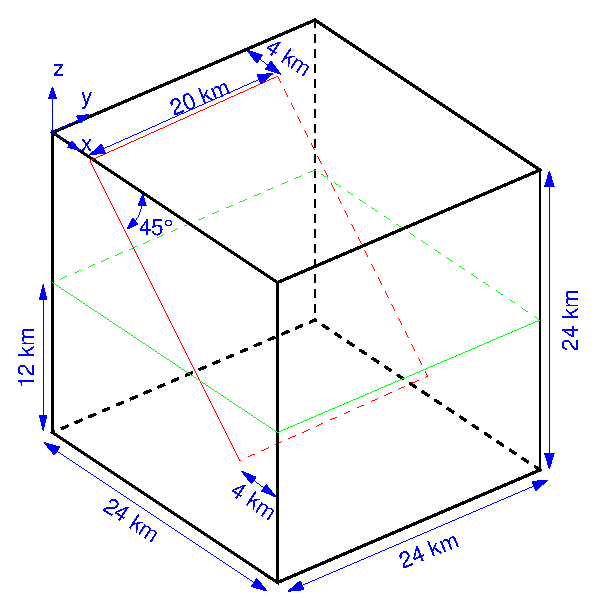
\includegraphics{figs/geometry}
    \caption{Geometry of model domain for simple model with strike-slip fault.}
  \end{center}
\end{figure}  

\subsubsection{Workflow}

The complete workflow used to create the input files for this tutorial
is shown in figure~\ref{fig:splitcube:workflow}. 

\begin{figure}[htbp]
  \begin{center}
    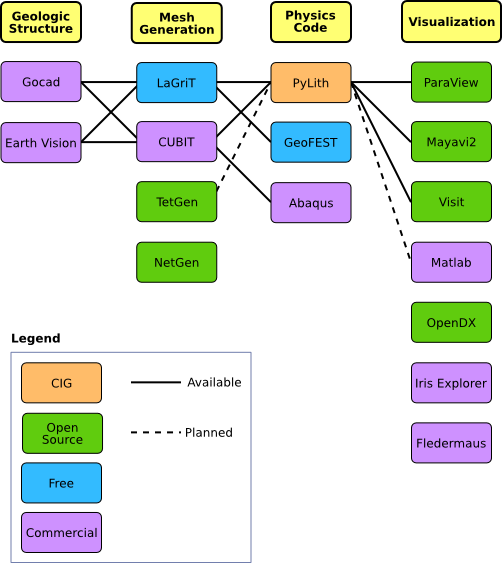
\includegraphics{figs/workflow}
    \caption{Workflow for setting up input files for example with
      simple strike-slip faylt.}
    \label{fig:splitcube:workflow}
  \end{center}
\end{figure}

\subsection{Download and unpack}

We will start by downloading the tutorial tarball and unpacking it.

\begin{enumerate}
\item Download the \href{http://www.geodynamics.org:8080/cig/Members/willic3/pylithusers/pylith0.8/pylith-0.8\_tutorials.tgz}{tutorial tarball}
  and unpack it in a location of your choosing.

  \begin{screen}
    \shellprompt\userinput{tar -zxvf pylith-0.8\_tutorials.tgz}
  \end{screen}
  
\item Go to the \directory{tutorials/splitcube} directory.
  The \directory{archive} directory contains all of the input and
  output files associated with this tutorial. We will copy input files
  from this directory into the \directory{workarea} directory. At each
  step, you can check to make sure your input and output agree with
  the files in the \directory{archive} directory. These files also
  allow you to start at an intermediate step as described in the next
  section.

  \begin{screen}
    \shellprompt\userinput{cd tutorials/splitcube}
  \end{screen}

\end{enumerate}

\subsection{Tutor}

Copy the \filename{tutor.py} script from the \directory{archive}
directory into the \directory{workarea} directory. 

\begin{tip}
  If you have run this tutorial previously, you may want to run
  \command{tutor.py} in mode "clean" with step "all" to clear out all
  old tutorial files.
\end{tip}

\begin{screen}
\shellprompt\userinput{cd workarea}
\shellprompt\userinput{cp ../archive/tutor.py .}
\shellprompt\userinput{./tutor.py -m clean -s all}
\end{screen}

\subsection{Generate the mesh}

In this step we will generate the finite-element mesh for the
benchmark problem using \application{NETGEN}.

\begin{enumerate}
\item In the \directory{splitcube/workarea} directory, run
  \command{tutor.py} for step "mesh" with mode "retrieve" to fetch the
  geometry file for \application{NETGEN}. You may also want to run
  \command{tutor.py} for this step with mode "clean" to clean out old
  files.

  \begin{screen}
    \shellprompt\userinput{./tutor.py -m retrieve -s mesh}
    \shellprompt\userinput{./tutor.py -m clean -s mesh}
  \end{screen}
  
\item Examine the \filename{splitcube.geo} file to see how the geometry
  for the problem is defined. Notice that the fault plan has
  been flagged with a boundary condition code. This will be
  used to associate boundary conditions with the fault surface and the
  associated nodes. We do not have to flag the lateral faces and top
  and bottom of the mesh because they are traction-free, which is a
  natural boundary condition in the finite-element formulation.
\item Start up \application{NETGEN} by running \command{ng}.

  \begin{screen}
    \shellprompt\userinput{ng}
  \end{screen}
  
\item Select \guimenu{File}\guiselect\guimenuitem{Load Geometry}
  and select \filename{splitcube.geo}.
\item Click on \guibutton{Generate Mesh}.
\item Export the mesh to a file named \filename{splitcube.netgen},
  making sure the export filetype is "Neutral format".
\item You can now exit \application{NETGEN}.
\end{enumerate}

\subsection{Setup simulation input files}

In this step we will setup the PyLith input files for the mesh and
boundary conditions.

\begin{enumerate}
\item Run \command{tutor.py} for step "setup" with mode "retrieve" to
  fetch files from the archive.

  \begin{screen}
    \shellprompt\userinput{./tutor.py -m retrieve -s setup}
  \end{screen}
  
\item We will use a simple Fortran utility to generate PyLith
  input files from the \application{NETGEN} output.

  \begin{description}
  \item[\command{readnetgen}] A Fortran program to read
    \application{NETGEN} neutral format and create several of the
    input files needed by PyLith.
  \end{description}
  
\item Run the \command{readnetgen} utility program to process the
  \application{NETGEN} output file into PyLith compatible input files.
  It will ask for a root filename, enter \filename{splitcube}. This
  utilitiy will generate the following files:
  \filename{splitcube.w01.wink}, \filename{splitcube.coord},
  \filename{splitcube.connect}, \filename{splitcube.bc},
  \filename{splitcube.1.fcoord}, \filename{splitcube.1.fbc}.

  \begin{screen}
    \shellprompt\userinput{../../utils/readnetgen}
    \prompt{\ Enter root name for all files.  Both input and}
    \prompt{\ output files will all have this prefix:}
    \userinput{splitcube}
  \end{screen}
  
\item The boundary conditions on the fault for this example are
  very simple. As a result, the \filename{splitcube.split} file was
  generated by hand. You should examine this file to see how a uniform
  right-lateral slip of 1.0 m is applied to the fault surface.

  \begin{warning}
    If you make any changes to \filename{splitcube.geo} or change the
    geometry within \application{NETGEN}, the split-node file
    \filename{splitcube.split} will no longer be correct and you will
    have to generate one yourself.  Note that it is also possible that
    a different version of \application{NETGEN} may provide a slightly
    different mesh, which would also be incompatible with the provided
    boundary conditions.
  \end{warning}
  
\item The external boundary conditions for this benchmark simply
  involve ... ADD STUFF HERE.

  \begin{warning}
    If you make any changes to \filename{splitcube.geo} or change the
    geometry within \application{NETGEN}, the boundary condition file
    \filename{splitcube.bc} will no longer be correct and you will
    have to generate one yourself.  Note that it is also possible that
    a different version of \application{NETGEN} may provide a slightly
    different mesh, which would also be incompatible with the provided
    boundary conditions.
  \end{warning}
\end{enumerate}

\subsection{Run the simulation on one processor}

In this step we will run the simulation on a single processor.

\begin{enumerate}
\item Run \command{tutor.py} for step "run1" with mode "retrieve" to
  fetch some parameter files from the archive.

  \begin{screen}
    \shellprompt\userinput{./tutor.py -m retrieve -s run1}
  \end{screen}
  
\item In \filename{splitcube.fuldat}, we have specified that we want
  full output at time steps 10, 50, and 100. We define two materials
  with elastic behavior in
  \filename{splitcube.prop}. In \filename{splitcube.statevar} we choose to
  include total stress, total strain, incremental stress, and
  incremental strain in the output. As defined in
  \filename{splitcube.time}, the simulation will have 100 time steps of
  0.1 year each.
\item Run the simulation by executing \userinput{runbm.py -n 1}, where
  the 1 refers to the number of processors.

  \begin{tip}
    All of the input is echoed in the file \filename{splitcube.ascii}.
    You can check to make sure your input is digested correctly by
    examining this file. For large problems, this file can be quite
    large. You can suppress creation of this file using the command
    line argument \option{--scanner.asciiOutput=none} flag. On the
    other hand, for debugging purposes in small problems, you may wish
    to output everything, including the computed results, in this file
    using \option{--scanner.asciiOutput=full}.
  \end{tip}
  
  \begin{screen}
    \shellprompt\userinput{./runbm.py -n 1}
  \end{screen}
\end{enumerate}

\subsection{Visualize the single processor run}

Now it is time to visualize the results of the simulation. By default,
PyLith writes simulation output using \href{http://help.avs.com/Express/doc/help/reference/dvmac/UCD\_Form.htm}{\application{AVS} UCD
  files}.
These can be read by several other visualization tools besides
\application{AVS}, e.g., \application{ParaView} and \application{Iris
  Explorer}. We will use the open-source application
\application{ParaView} to visualize the results.
    
\begin{enumerate}
\item If necessary, run \command{tutor.py} for step "viz1" with mode
  "retrieve" to fetch the simulation output from the archive.

  \begin{screen}
    \shellprompt\userinput{./tutor.py -m retrieve -s viz1}
  \end{screen}
  
\item PyLith does not write complete UCD files. So the first step is
  to combine the mesh topology information with the output at a given
  time step into a complete UCD file. For example, use \command{cat}
  to merge the nodal coordinates file
  (\filename{splitcube\_1.0.mesh.inp}) and the nodal displacements at
  time step 10 file (\filename{splitcube\_1.0.mesh.time.00010.inp}) into
  \filename{splitcube\_1.0.mesh.t00010.inp}.

  \begin{screen}
    \shellprompt\userinput{cat splitcube\_1.0.mesh.inp splitcube\_1.0.mesh.time.00010.inp \(\backslash\)}
    \userinput{> splitcube\_1.0.mesh.t00010.inp}
\end{screen}

\item Start \application{ParaView} by executing \command{paraview}.

  \begin{screen}
    \shellprompt\userinput{paraview}
  \end{screen}
  
\item Load the UCD file that you just created by selecting
  \guimenu{File}\guiselect\guimenuitem{Open Data}. Select the file in
  the dialog box and the click the \guibutton{Open} button. Click the
  \guibutton{Accept} button. You should see a color rendering of the x
  displacements. You can use the mouse to rotate, translate, and zoom.
  Your image should look similar to the one in
  figure~\ref{fig::splitcube:xdisp:t10}.
        
  \begin{figure}[htbp]
    \begin{center}
      %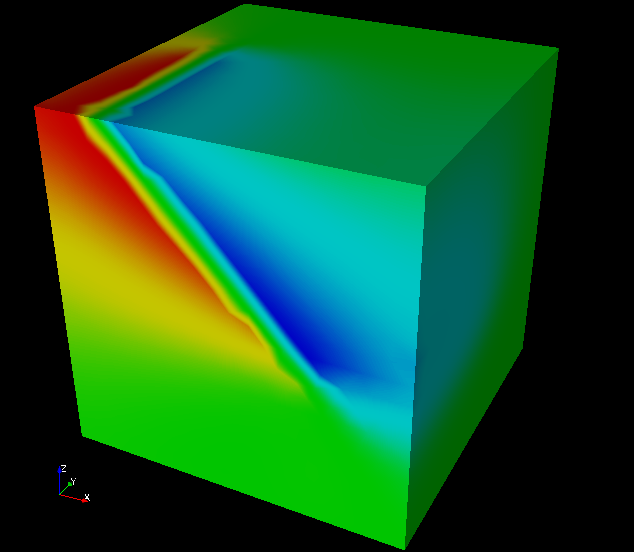
\includegraphics{figs/xdisp_t10}
      \caption{ParaView rendering of displacement in x-direction at
          time step 10 (10 yrs after imposed dislocation) for the
          simple strike-slip example.}
      \label{fig:splitcube:xdisp:t10}
    \end{center}
  \end{figure}
  
\item In the \guibutton{Display} tab, you can change several options,
  such as including a color bar, coloring a different component,
  interpolating colors, and changing the color map.
\item Let's show the displacements as vectors. Click on the calculator
  icon, and add the three displacement components together. Enter
  \begin{screen}
  XDispl*iHat + YDispl*jHat + ZDispl*kHat
  \end{screen}
  in the \guimenuitem{Calculator}
  box. Note the variable names are available by clicking on the
  \guibutton{scalars} button and the \guibutton{iHat},
  \guibutton{jHat}, \guibutton{kHat} buttons are on the right side of
  the top row. Click on the \guibutton{Accept} button. To show the
  dataset as vectors, click on the \guibutton{glyph} button (looks
  like several dots) in the toolbar. After clicking the
  \guibutton{Accept} button, you should have a vector plot. You can
  turn on/off other datasets by clicking on the eye icon to the left
  of the dataset name. If you color the surfaces using the
  x-displacements field while also making the displacement vectors
  visible (colored using property), you should see an image similar to
  the one in figure~\ref{fig:splitcube:xdisp:vec:t10}.

  \begin{figure}[htbp]
    \begin{center}
      %\includegraphics{figs/splitcube_xdisp_vec_t10}
      \caption{ParaView rendering of displacement in x-direction and
        displacement vectors at time step 10 (10 yrs after imposed
        dislocation) for the simple strike-slip example.}
      \label{fig:splitcube:xdisp:vec:t10}
    \end{center}
  \end{figure}      

\end{enumerate}

\subsection{Run the simulation on two processors}

In this step we will run the simulation on two processors. Even if
your machine only has one processor, a "multprocessor" job will run as
multiple processes on the single processor. In such cases, the job
will run slightly slower than the single processor run, but the two
processes will behave independently as if they are on different
processors.

\begin{enumerate}
\item Run \command{tutor.py} for step "run2" with mode "retrieve" to
  make sure all parameter files are available.

  \begin{screen}
    \shellprompt\userinput{./tutor.py -m retrieve -s run2}
  \end{screen}
  
\item The parameter files are the same as those in the single
  processor run. The \command{runbm} script will automatically take
  care of duplicating these files so that there is one for each
  processor.
\item Run the simulation by executing \command{runbm.py -n 2}, where
  the 2 refers to the number of processors.

  \begin{screen}
    \shellprompt\userinput{./runbm.py -n 2}
  \end{screen}
\end{enumerate}

\subsection{Visualize the two processor run}

PyLith does not currently support parallel output, so each processor
writes its UCD output to a different file. This means that you need to
form complete UCD files for each processor and then load each one into
\application{ParaView}.

\begin{enumerate}
\item If necessary, run \command{tutor.py} for step "viz2" with mode
  "retrieve" to fetch the simulation output from the archive.

  \begin{screen}
    \shellprompt\userinput{./tutor.py -m retrieve -s viz2}
  \end{screen}
  
\item As in the case of the single processor run, the first step is to
  combine the mesh topology information with the output at a given
  time step into a complete UCD file. Because PyLith writes the output
  from each processor into a different file, we must run \command{cat}
  twice to create UCD files for each processor.

  \begin{screen}
    \shellprompt\userinput{cat splitcube\_2.0.mesh.inp splitcube\_2.0.mesh.time.00010.inp \(\backslash\)}
      \userinput{> splitcube\_2.0.mesh.t00010.inp}
    \shellprompt\userinput{cat splitcube\_2.1.mesh.inp splitcube\_2.1.mesh.time.00010.inp \(\backslash\)}
      \userinput{> splitcube\_2.1.mesh.t00010.inp}
  \end{screen}

\item Start \application{ParaView} by executing \command{paraview}.

  \begin{screen}
    \shellprompt\userinput{paraview}
  \end{screen}
  
\item Load the UCD files that you just created by selecting
  \guimenu{File}\guiselect\guimenuitem{Open Data}. Select the file in
  the dialog box and the click the \guibutton{Open} button. Click the
  \guibutton{Accept} button. You can now visualize the datasets just
  like you did for the single processor case.
\item You can merge the datasets from the different processors by
  selecting \guimenu{Filter}\guiselect\guimenuitem{Append}. Doing so
  will allow you to operate on the data from all of the processors
  simultaneously instead of having to repeat any processing for every
  processor.
\end{enumerate}

\section{Tutorial Using Reverse-Slip Without Gravity Benchmark}

\subsection{Overview}

In this tutorial, we will walk through the steps necessary to
construct, run, and view the results of a benchmark problem involving
reverse slip on a dipping fault. This problem examines the
viscoelastic (Maxwell) relaxation of stress from a single, finite,
reverse-slip earthquake in 3-D without body forces.


\subsection{Problem Description}

The model domain is a cube with edges 24 km long (0 km $\leq$ x $\leq$
24 km; 0 km $\leq$ y $\leq$ 24 km; -24 km $\leq$ z $\leq$ 0) and
is composed of two materials. One material occupies the top-half of
the domain, -12 km $\leq$ z $\leq$ 0 km, while the other occupies
the lower half, -24 km $\leq$ z $<$ 12 km. Both materials are Poisson
solids with Lame's constants ($\mu$ and $\lambda$) equal to 30 GPa and
Maxwell viscoelastic properties. The top layer has a viscosity of
$10^25$ Pa-s (and is essentially elastic) while the bottom layer has a
viscosity of $10^18$ Pa-s.

The reverse fault dips at an angle of 45 degrees. The top of the fault
sits at x = 4 km with the bottom of the fault at x = 20 km. The fault
surface is confined to the region 0 km $\leq$ y $\leq$ 16 km and -16
km $\leq$ z $\leq$ 0 km. The slip distribution is 1.0 m of uniform
thrust motion for -12 km $\leq$ z with a linear taper to 0 at z = -16
km.

The plane y=0 is a plane of symmetry, so the y-DOF displacements on
this face are zero. The boundary conditions on the other lateral faces
and bottom of the mesh are the displacements from the analytical
elastic solution. These displacements are held fixed through time.

\begin{figure}
  \begin{center}
    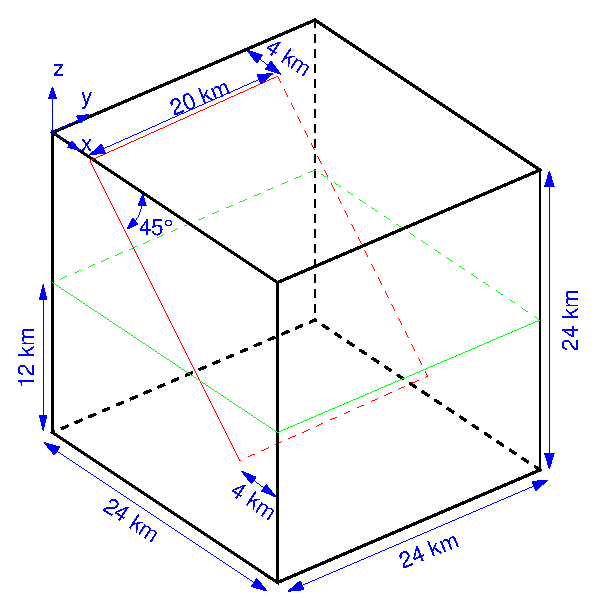
\includegraphics{figs/geometry}
    \caption{Geometry of model domain for reverse-slip benchmark.}
  \end{center}
\end{figure}  

\subsubsection{Workflow}

The complete workflow used to create the input files for this tutorial
is shown in figure~\ref{fig:bmrsnog:workflow}. Because some of the
steps involve commercial software (e.g., Matlab), we will skip those
steps in this tutorial.

\begin{figure}[htbp]
  \begin{center}
    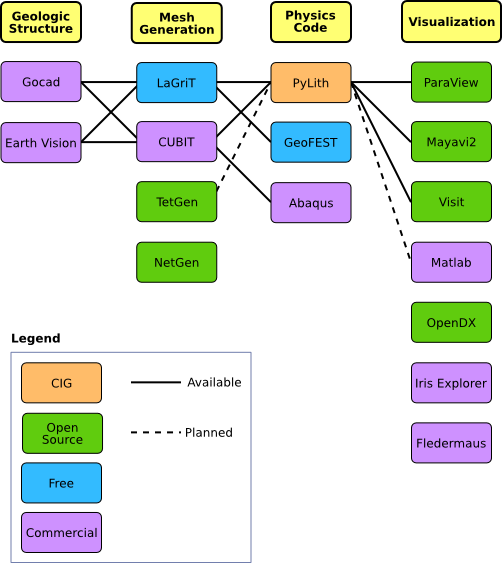
\includegraphics{figs/workflow}
    \caption{Workflow for setting up input files for benchmark with reverse
      slip and no gravity.}
    \label{fig:bmrsnog:workflow}
  \end{center}
\end{figure}

\subsection{Download and unpack}

We will start by downloading the tutorial tarball and unpacking it.

\begin{enumerate}
\item Download the \href{http://www.geodynamics.org:8080/cig/Members/willic3/pylithusers/pylith0.8/pylith-0.8\_tutorials.tgz}{tutorial
    tarball}
  and unpack it in a location of your choosing.

  \begin{screen}
    \shellprompt\userinput{tar -zxvf pylith-0.8\_tutorials.tgz}
  \end{screen}
  
\item Go to the \directory{tutorials/reversenog} directory.
  The \directory{archive} directory contains all of the input and
  output files associated with this tutorial. We will copy input files
  from this directory into the \directory{workarea} directory. At each
  step, you can check to make sure your input and output agree with
  the files in the \directory{archive} directory. These files also
  allow you to start at an intermediate step as described in the next
  section.

  \begin{screen}
    \shellprompt\userinput{cd tutorials/reversenog}
  \end{screen}

\end{enumerate}

\subsection{Tutor}

Copy the \filename{tutor.py} script from the \directory{archive}
directory into the \directory{workarea} directory. 

\begin{tip}
  If you have run this tutorial previously, you may want to run
  \command{tutor.py} in mode "clean" with step "all" to clear out all
  old tutorial files.
\end{tip}

\begin{screen}
\shellprompt\userinput{cd workarea}
\shellprompt\userinput{cp ../archive/tutor.py .}
\shellprompt\userinput{./tutor.py -m clean -s all}
\end{screen}

\subsection{Generate the mesh}

In this step we will generate the finite-element mesh for the
benchmark problem using \application{NETGEN}.

\begin{enumerate}
\item In the \directory{reversenog/workarea} directory, run
  \command{tutor.py} for step "mesh" with mode "retrieve" to fetch the
  geometry file for \application{NETGEN}. You may also want to run
  \command{tutor.py} for this step with mode "clean" to clean out old
  files.

  \begin{screen}
    \shellprompt\userinput{./tutor.py -m retrieve -s mesh}
    \shellprompt\userinput{./tutor.py -m clean -s mesh}
  \end{screen}
  
\item Examine the \filename{bmrsnog.geo} file to see how the geometry
  for the problem is defined. Notice that the different planes have
  been flagged with different boundary condition codes. These will be
  used to associate boundary conditions with surfaces and element
  nodes.
\item Start up \application{NETGEN} by running \command{ng}.

  \begin{screen}
    \shellprompt\userinput{ng}
  \end{screen}
  
\item Select \guimenu{File}\guiselect\guimenuitem{Load Geometry}
  and select \filename{bmrsnog.geo}.
\item Click on \guibutton{Generate Mesh}.
\item Export the mesh to a file named \filename{bmrsnog.netgen},
  making sure the export filetype is "Neutral format".
\item You can now exit \application{NETGEN}.
\end{enumerate}

\subsection{Setup simulation input files}

In this step we will setup the PyLith input files for the mesh and
boundary conditions.

\begin{enumerate}
\item Run \command{tutor.py} for step "setup" with mode "retrieve" to
  fetch files from the archive.

  \begin{screen}
    \shellprompt\userinput{./tutor.py -m retrieve -s setup}
  \end{screen}
  
\item We will use two simple Fortran utilities to generate PyLith
  input files from the \application{NETGEN} output.

  \begin{description}
  \item[\command{readnetgen}] A Fortran program to read
    \application{NETGEN} neutral format and create several of the
    input files needed by PyLith.
  \item[\command{faultcalc}] A Fortran program to compute split node
    displacements using second order polynomials over specified
    regions.
  \end{description}
  
\item Run the \command{readnetgen} utility program to process the
  \application{NETGEN} output file into PyLith compatible input files.
  It will ask for a root filename, enter \filename{bmrsnog}. This
  utilitiy will generate the following files:
  \filename{bmrsnog.w01.wink}, \filename{bmrsnog.coord},
  \filename{bmrsnog.connect}, \filename{bmrsnog.bc},
  \filename{bmrsnog.1.fcoord}, \filename{bmrsnog.1.fbc}.

  \begin{screen}
    \shellprompt\userinput{../../utils/readnetgen}
    \prompt{\ Enter root name for all files.  Both input and}
    \prompt{\ output files will all have this prefix:}
    \userinput{bmrsnog}
  \end{screen}
  
\item The boundary conditions on the fault for this benchmark are
  somewhat complex. The utility program \command{faultcalc} creates
  split node boundary conditions over specified regions, using
  functions based on second degree polynomials. The
  \command{readnetgen} program has already produced the main input for
  \command{faultcalc} -- split node definitions in
  \filename{bmrsnog.1.fbc} and nodal coordinates in
  \filename{bmrsnog.coord}. The file \filename{bmrsnog.fault.par}
  contains the polynomial coefficients for this benchmark problem. Run
  \command{faultcalc} to get the \filename{bmrsnog.split} file that
  PyLith needs as input.

  \begin{screen}
    \shellprompt\userinput{../../utils/faultcalc p=bmrsnog.fault.par n=bmrsnog.coord \(\backslash\)}
      \userinput{i=bmrsnog.1.fbc o=bmrsnog.split}
  \end{screen}
  
\item The external boundary conditions for this benchmark are also
  complicated and require computing the displacements for the
  analytical elastic solution at each finite element node on the
  external boundaries. The file specifying these boundary conditions,
  \filename{bmrsnog.bc}, was produced with \command{readnetgen} using
  the \filename{bmrsnog.aux} file (which contains precomputed
  displacements for the external boundaries for the mesh produced from
  the \filename{bmrsnog.geo} geometry).

  \begin{warning}
    If you make any changes to \filename{bmrsnog.geo} or change the
    geometry within \application{NETGEN}, the boundary condition file
    \filename{bmrsnog.bc} will no longer be correct and you will have
    to generate one yourself.  Note that it is also possible that a
    different version of \application{NETGEN} may provide a slightly
    different mesh, which would also be incompatible with the provided
    boundary conditions.
  \end{warning}
\end{enumerate}

\subsection{Run the simulation on one processor}

In this step we will run the simulation on a single processor.

\begin{enumerate}
\item Run \command{tutor.py} for step "run1" with mode "retrieve" to
  fetch some parameter files from the archive.

  \begin{screen}
    \shellprompt\userinput{./tutor.py -m retrieve -s run1}
  \end{screen}
  
\item In \filename{bmrsnog.fuldat}, we have specified that we want
  full output at time steps 10, 50, and 100. We define six materials
  with both elastic and viscoelastic behavior in
  \filename{bmrsnog.prop}. In \filename{bmrsnog.statevar} we choose to
  include total stress, total strain, incremental stress, and
  incremental strain in the output. As defined in
  \filename{bmrsnog.time}, the simulation will have 100 time steps of
  0.1 year each.
\item Run the simulation by executing \userinput{runbm.py -n 1}, where
  the 1 refers to the number of processors.

  \begin{tip}
    All of the input is echoed in the file \filename{bmrsnog.ascii}.
    You can check to make sure your input is digested correctly by
    examining this file. For large problems, this file can be quite
    large. You can suppress creation of this file using the command
    line argument \option{--scanner.asciiOutput=none} flag. On the
    other hand, for debugging purposes in small problems, you may wish
    to output everything, including the computed results, in this file
    using \option{--scanner.asciiOutput=full}.
  \end{tip}
  
  \begin{screen}
    \shellprompt\userinput{./runbm.py -n 1}
  \end{screen}
\end{enumerate}

\subsection{Visualize the single processor run}

Now it is time to visualize the results of the simulation. By default,
PyLith writes simulation output using
\href{http://help.avs.com/Express/doc/help/reference/dvmac/UCD\_Form.htm}{\application{AVS}
  UCD files}.  These can be read by several other visualization tools
besides \application{AVS}, e.g., \application{ParaView} and
\application{Iris Explorer}. We will use the open-source application
\application{ParaView} to visualize the results.
    
\begin{enumerate}
\item If necessary, run \command{tutor.py} for step "viz1" with mode
  "retrieve" to fetch the simulation output from the archive.

  \begin{screen}
    \shellprompt\userinput{./tutor.py -m retrieve -s viz1}
  \end{screen}
  
\item PyLith does not write complete UCD files. So the first step is
  to combine the mesh topology information with the output at a given
  time step into a complete UCD file. For example, use \command{cat}
  to merge the nodal coordinates file
  (\filename{bmrsnog\_1.0.mesh.inp}) and the nodal displacements at
  time step 10 file (\filename{bmrsnog\_1.0.mesh.time.00010.inp}) into
  \filename{bmrsnog\_1.0.mesh.t00010.inp}.

  \begin{screen}
    \shellprompt\userinput{cat bmrsnog\_1.0.mesh.inp bmrsnog\_1.0.mesh.time.00010.inp \(\backslash\)}
    \userinput{> bmrsnog\_1.0.mesh.t00010.inp}
\end{screen}

\item Start \application{ParaView} by executing \command{paraview}.

  \begin{screen}
    \shellprompt\userinput{paraview}
  \end{screen}
  
\item Load the UCD file that you just created by selecting
  \guimenu{File}\guiselect\guimenuitem{Open Data}. Select the file in
  the dialog box and the click the \guibutton{Open} button. Click the
  \guibutton{Accept} button. You should see a color rendering of the x
  displacements. You can use the mouse to rotate, translate, and zoom.
  Your image should look similar to the one in
  figure~\ref{fig::bmrsnog:xdisp:t10}.
        
  \begin{figure}[htbp]
    \begin{center}
      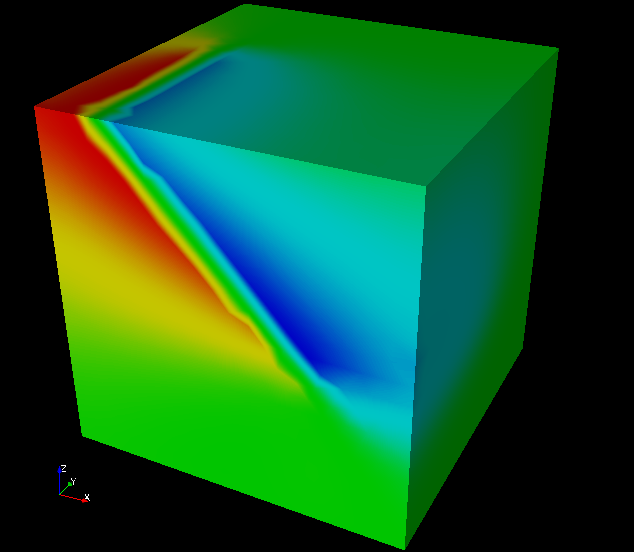
\includegraphics{figs/xdisp_t10}
      \caption{ParaView rendering of displacement in x-direction at
          time step 10 (10 yrs after imposed dislocation) for the
          reverse slip without gravity benchmark.}
      \label{fig:bmrsnog:xdisp:t10}
    \end{center}
  \end{figure}
  
\item In the \guibutton{Display} tab, you can change several options,
  such as including a color bar, coloring a different component,
  interpolating colors, and changing the color map.
\item Let's show the displacements as vectors. Click on the calculator
  icon, and add the three displacement components together. Enter
  \begin{screen}
  XDispl*iHat+YDispl*jHat+ZDispl*kHat
  \end{screen}
  in the \guimenuitem{Calculator} box. Note the variable names are
  available by clicking on the \guibutton{scalars} button and the
  \guibutton{iHat}, \guibutton{jHat}, \guibutton{kHat} buttons are on
  the right side of the top row. Click on the \guibutton{Accept}
  button. To show the dataset as vectors, click on the
  \guibutton{glyph} button (looks like several dots) in the toolbar.
  After clicking the \guibutton{Accept} button, you should have a
  vector plot. You can turn on/off other datasets by clicking on the
  eye icon to the left of the dataset name. If you color the surfaces
  using the x-displacements field while also making the displacement
  vectors visible (colored using property), you should see an image
  similar to the one in figure~\ref{fig:bmrsnog:xdisp:vec:t10}.

  \begin{figure}[htbp]
    \begin{center}
      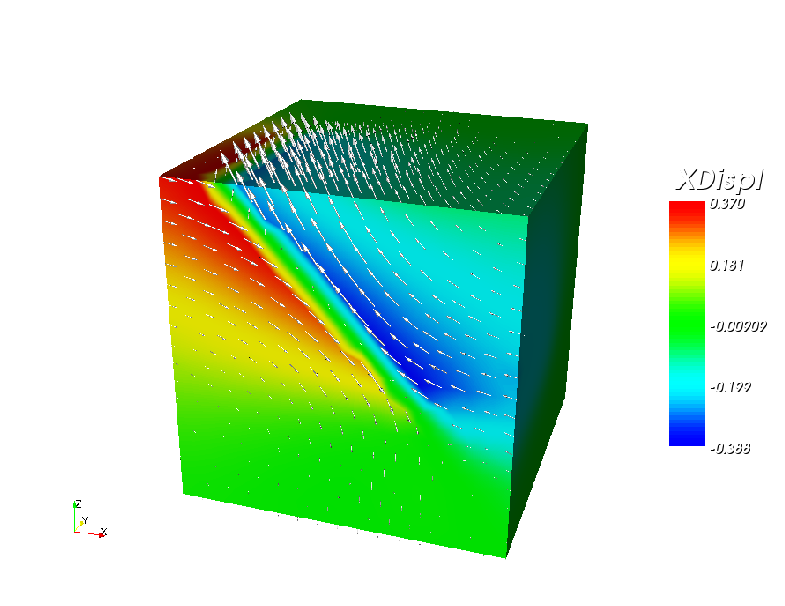
\includegraphics{figs/xdisp_vec_t10}
      \caption{ParaView rendering of displacement in x-direction and
        displacement vectors at time step 10 (10 yrs after imposed
        dislocation) for the reverse slip without gravity
        benchmark.}
      \label{fig:bmrsnog:xdisp:vec:t10}
    \end{center}
  \end{figure}      

\end{enumerate}

\subsection{Run the simulation on two processors}

In this step we will run the simulation on two processors. Even if
your machine only has one processor, a "multprocessor" job will run as
multiple processes on the single processor. In such cases, the job
will run slightly slower than the single processor run, but the two
processes will behave independently as if they are on different
processors.

\begin{enumerate}
\item Run \command{tutor.py} for step "run2" with mode "retrieve" to
  make sure all parameter files are available.

  \begin{screen}
    \shellprompt\userinput{./tutor.py -m retrieve -s run2}
  \end{screen}
  
\item The parameter files are the same as those in the single
  processor run. The \command{runbm} script will automatically take
  care of duplicating these files so that there is one for each
  processor.
\item Run the simulation by executing \command{runbm.py -n 2}, where
  the 2 refers to the number of processors.

  \begin{screen}
    \shellprompt\userinput{./runbm.py -n 2}
  \end{screen}
\end{enumerate}

\subsection{Visualize the two processor run}

PyLith does not currently support parallel output, so each processor
writes its UCD output to a different file. This means that you need to
form complete UCD files for each processor and then load each one into
\application{ParaView}.

\begin{enumerate}
\item If necessary, run \command{tutor.py} for step "viz2" with mode
  "retrieve" to fetch the simulation output from the archive.

  \begin{screen}
    \shellprompt\userinput{./tutor.py -m retrieve -s viz2}
  \end{screen}
  
\item As in the case of the single processor run, the first step is to
  combine the mesh topology information with the output at a given
  time step into a complete UCD file. Because PyLith writes the output
  from each processor into a different file, we must run \command{cat}
  twice to create UCD files for each processor.

  \begin{screen}
    \shellprompt\userinput{cat bmrsnog\_2.0.mesh.inp bmrsnog\_2.0.mesh.time.00010.inp \(\backslash\)}
      \userinput{> bmrsnog\_2.0.mesh.t00010.inp}
    \shellprompt\userinput{cat bmrsnog\_2.1.mesh.inp bmrsnog\_2.1.mesh.time.00010.inp \(\backslash\)}
      \userinput{> bmrsnog\_2.1.mesh.t00010.inp}
  \end{screen}

\item Start \application{ParaView} by executing \command{paraview}.

  \begin{screen}
    \shellprompt\userinput{paraview}
  \end{screen}
  
\item Load the UCD files that you just created by selecting
  \guimenu{File}\guiselect\guimenuitem{Open Data}. Select the file in
  the dialog box and the click the \guibutton{Open} button. Click the
  \guibutton{Accept} button. You can now visualize the datasets just
  like you did for the single processor case.
\item You can merge the datasets from the different processors by
  selecting \guimenu{Filter}\guiselect\guimenuitem{Append}. Doing so
  will allow you to operate on the data from all of the processors
  simultaneously instead of having to repeat any processing for every
  processor.
\end{enumerate}



\appendix
%dummy comment inserted by tex2lyx to ensure that this paragraph is not empty
\chapter{File Formats}

\section{Input Files}

PyLith gathers its input from several different types of files. All of
these area ASCII files and can include comment lines that begin with
'\#'. Note that the placement of comments is restricted to certain
locations in some files (see the discussion of each file format for
more information).

% REQUIRED INPUT FILES

\subsection{xx.coord}

The \filename{xx.coord} file contains the coordinates of all of the
vertices in the finite-element mesh.

\begin{figure}[htbp]
  \begin{center}
    \verbatiminput{data/xx.coord}
    \caption{Format of \filename{xx.coord} files.}
  \end{center}
\end{figure}

\subsection{xx.connect}

The \filename{xx.connect} file contains the finite-element mesh
topology and material type information, including the element type,
material type, and the lists of vertices for each element.

\begin{figure}[htbp]
  \begin{center}
    \verbatiminput{data/xx.connect}
    \caption{Format of \filename{xx.connect} files.}
  \end{center}
\end{figure}  

\subsection{xx.bc}

The \filename{xx.bc} file specifies the displacements, velocity,
and/or forces applied to vertices on the boundaries.

\begin{figure}[htbp]
  \begin{center}
    \verbatiminput{data/xx.bc}
    \caption{Format of \filename{xx.bc} files.}
  \end{center}
\end{figure}

\subsection{xx.time}

The \filename{xx.time} file specifies the time stepping parameters for
the simulation.

\begin{warning}
  The convergence criteria depend on the type of solution and material
  models. The time step for a linear elastic problem is much different
  than that for a nonlinear or time-dependent problem.
\end{warning}

\begin{figure}[htbp]
  \begin{center}
    \verbatiminput{data/xx.time}
    \caption{Format of \filename{xx.time} files.}
  \end{center}
\end{figure}

\subsection{xx.prop}

The \filename{xx.prop} file specifies the properties for each material
model in the problem.

\begin{warning}
  The materials must be listed in order according to the material
  number assigned to the elements in \filename{xx.connect}.
\end{warning}

\begin{figure}[htbp]
  \begin{center}
    \verbatiminput{data/xx.prop}
    \caption{Format of \filename{xx.prop} files.}
  \end{center}
\end{figure}

\subsection{xx.statevar}

The \filename{xx.statevar} file specifies which state variables are to
be included in the output of the elastic and time dependent solutions.

\begin{figure}[htbp]
  \begin{center}
    \verbatiminput{data/xx.statevar}
    \caption{Format of \filename{xx.statevar} files.}
  \end{center}
\end{figure}

% OPTIONAL INPUT FILES

\subsection{xx.split}

The \filename{xx.split} file specifies the split node information for
modeling dislocations. Dislocations may be used in simulating slip on
faults as well as dike intrusions.

\begin{figure}[htbp]
  \begin{center}
    \verbatiminput{xx.split}
    \caption{Format of \filename{xx.split} files.}
  \end{center}
\end{figure}

\subsection{xx.fuldat}

The \filename{xx.fuldat} file lists the time step numbers at which
full output is desired. The elastic solution (time step 0) is always
included in the output. This file is required for time-dependent
problems.

\begin{figure}[htbp]
  \begin{center}
    \verbatiminput{xx.fuldat}
    \caption{Format of \filename{xx.time} files.}
  \end{center}
\end{figure}

\subsection{xx.skew}

The \filename{xx.skew} file specifies local coordinate systems for
nodes. The local coordinate system is specified using two Euler angles
that rotate the local coordinate system to the global coordinate
system.

The applied coordinate rotations apply to all boundary conditions
associated with the nodes listed in the file. These are useful, for
example, if it is desired to apply boundary conditions in a direction
normal or tangential to a side of the mesh when the side does not
align with the global coordinate directions.  Similarly, skew
conditions could be used when specifying slip on a fault that lies at
an angle to the global coordinates.

\begin{figure}[htbp]
  \begin{center}
    \verbatiminput{xx.skew}
    \caption{Format of \filename{xx.time} files.}
  \end{center}
\end{figure}

\subsection{xx.keyval}

The \filename{xx.keyval} file specifies some simple parameter
settings.

\subsubsection{Winkler forces}

Scaling factors can be applied to Winkler forces, permitting a quick
and easy way to change the density or gravitational acceleration when
Winkler forces are used to simulate gravity.

\paragraph{Quadrature order}

\begin{description}
\item[Full] Quadrature order that should give the exact element
  matrices when the elements are geometrically undistorted.
\item[Reduced] Quadrature order that is one order less than full
  quadrature. Note that for linear tetrahedra full and reduced
  quadrature are equivalent (single integration point).

  \begin{warning}
    Use with caution as reduced quadrature can lead to numerical
    instabilities.
  \end{warning}
  
\item[Selective] Uses Hughes' b-bar formulation to perform reduced
  quadrature on the dilatational parts of the strain-displacement
  matrix.  This can be useful in nearly-incompressible problems.
\end{description}

\paragraph{Prestresses}

Gravitational prestresses can be computed automatically. In such
cases, the elastic properties in the prestress calculation can be set
to uniform values independent of the parameters for any of the
material models. When gravity is being used and prestresses are not
computed automatically, each prestress component can be scaled
independently. Reading prestresses from files is presently disabled.

\begin{figure}[htbp]
  \begin{center}
    \verbatiminput{xx.keyval}
  \caption{Format of \filename{xx.keyval} files.}
  \end{center}
\end{figure}

\subsection{xx.hist}

The \filename{xx.hist} files provide time histories for use in
boundary conditions.

\begin{figure}
  \begin{center}
    \verbatiminput{xx.hist}
    \caption{Format of \filename{xx.hist} files.}
  \end{center}
\end{figure}

\subsection{xx.wink}

The \filename{xx.wink} file specifies Winkler elements, which may be
used as spring foundations in the simulation of gravity.

\begin{figure}
  \begin{center}
    \verbatiminput{xx.wink}
    \caption{Format of \filename{xx.wink} files.}
  \end{center}
\end{figure}
 \chapter{Material Models}

\section{Effective Stress Function Formulation for a Maxwell Linear
Viscoelastic Material}

\subsection{Determination of stresses}

The element stresses are
\begin{equation}
  \text{figs/ml-eq1.eps}
\end{equation}
where ?? is the total strain and $\text{ml-inlineeq1}$ is the initial
stress. In terms of the deviatoric stress,
\begin{equation}
  \text{figs/ml-eq2.eps}
\end{equation}
where
\begin{equation}
  \text{figs/ml-eq3.eps}
\end{equation}
and the mean stress and strain are given by
\begin{equation}
  \text{figs/ml-eq4.eps}
\end{equation}
Equation~(2) [REPLACE WITH REF] may also be written as
\begin{equation}
  \text{figs/ml-eq4.eps}
\end{equation}
where
\begin{equation}
  \text{figs/ml-eq6.eps}
\end{equation}
The creep strain increment is approximated using
\begin{equation}
  \text{figs/ml-eq7.eps}
\end{equation}
where, using the $\alpha$-method of time integration,
\begin{equation}
  \text{figs/ml-eq8.eps}
\end{equation}
and
\begin{equation}
  \text{figs/ml-eq9.eps}
\end{equation}
where
\begin{equation}
  \text{figs/ml-eq10.eps}
\end{equation}
and
\begin{equation}
  \text{figs/ml-eq11.eps}
\end{equation}
For a linear Maxwell viscoelastic material
\begin{equation}
  \text{figs/ml-eq12.eps}
\end{equation}
Therefore,
\begin{equation}
  \text{figs/ml-eq13.eps}
\end{equation}
Subsituting (8), (12), and (13) into (5) [REPLACE WITH REFS], we obtain
\begin{equation}
  \text{figs/ml-eq14.eps}
\end{equation}
Solving for  $\text{figs/ml-inlineeq2}$,
\begin{equation}
  \text{figs/ml-eq15.eps}
\end{equation}
In this case it is possible to solve directly for the deviatoric
stresses, and the effective stress function approach is not needed. To
obtain the total stress, we simply use
\begin{equation}
  \text{figs/ml-eq16.eps}
\end{equation}

\subsection{Tangent stress-strain relation}

It is now necessary to provide a relationship for the viscoelastic
tangent material matrix. If we use vectors composed of the stresses
and tensor strains, this relationship is
\begin{equation}
  \text{figs/ml-eq17.eps}
\end{equation}
In terms of the vectors, we have
\begin{equation}
  \text{figs/ml-eq18.eps}
\end{equation}
Therefore,
\begin{equation}
  \text{figs/ml-eq19.eps}
\end{equation}
Using the chain rule,
\begin{equation}
  \text{figs/ml-eq20.eps}
\end{equation}
From (6) [REPLACE WITH REF], we obtain
\begin{equation}
  \text{figs/ml-eq21.eps}
\end{equation}
and from (3) [REPLACE WITH REF]
\begin{equation}
  \text{figs/ml-eq22.eps}
\end{equation}
Finally, from (15) [REPLACE WITH REF], we have
\begin{equation}
  \text{figs/ml-eq23.eps}
\end{equation}
From (19) [REPLACE WITH REF], the final material matrix relating
stress and tensor strain is
\begin{equation}
  \text{figs/ml-eq24.eps}
\end{equation}
Note that the coefficient of the second matrix approaches $E/3(1+\nu)$
as $\eta$ goes to infinity. Since finite element computations
typically use engineering strain measures, the matrix that is actually
used is
\begin{equation}
  \text{figs/ml-eq25.eps}
\end{equation}
To check the results we make sure that the regular elastic
constitutive matrix is obtained for selected terms in the case where
$\eta$ goes to infinity.
\begin{equation}
  \text{figs/ml-eq26.eps}
\end{equation}
This is consistent with the regular elasticity matrix, and equation
(25) [REPLACE WITH REF] should thus be used when forming the stiffness
matrix.



\chapter{PyLith Software License}

Copyright (C) 2004-2006 Rensselaer Polytechnic Institute

Permission is hereby granted, free of charge, to any person obtaining
a copy of this software and associated documentation files (the
"Software"), to deal in the Software without restriction, including
without limitation the rights to use, copy, modify, merge, publish,
distribute, sublicense, and/or sell copies of the Software, and to
permit persons to whom the Software is furnished to do so, subject to
the following conditions:

The above copyright notice and this permission notice shall be
included in all copies or substantial portions of the Software.

THE SOFTWARE IS PROVIDED "AS IS", WITHOUT WARRANTY OF ANY KIND,
EXPRESS OR IMPLIED, INCLUDING BUT NOT LIMITED TO THE WARRANTIES OF
MERCHANTABILITY, FITNESS FOR A PARTICULAR PURPOSE AND
NONINFRINGEMENT. IN NO EVENT SHALL THE AUTHORS OR COPYRIGHT HOLDERS BE
LIABLE FOR ANY CLAIM, DAMAGES OR OTHER LIABILITY, WHETHER IN AN ACTION
OF CONTRACT, TORT OR OTHERWISE, ARISING FROM, OUT OF OR IN CONNECTION
WITH THE SOFTWARE OR THE USE OR OTHER DEALINGS IN THE SOFTWARE.


\begin{thebibliography}{1}
\bibitem{Williams:2006}Williams, C. A. (2006), Development of a package
for modeling stress in the lithosphere, Eos Trans. AGU, 87(36), Jt.
Assem. Suppl., Abstract T24A-01 Invited.

\bibitem{Williams:etal:2005}Williams, C. A., B. Aagaard, M. G. Knepley
(2005), Development of software for studying earthquakes across multiple
spatial and temporal scales by coupling quasi-static and dynamic simulations,
Eos Trans. AGU, 86 (52), Fall Meet. Suppl., Abstract S53A-1072.

\bibitem{Kojic:Bathe:1987}Kojic, M. and K.-J. Bathe (1987), The 'Effective
Stress-Function' Algorithm for Thermo-Elasto-Plasticity and Creep,
\emph{Int. J. Num. Meth. Eng.}, 24, 1509-1532.
\end{thebibliography}

\end{document}
